% options:
% thesis=B bachelor's thesis
% thesis=M master's thesis
% czech thesis in Czech language
% english thesis in English language
% hidelinks remove colour boxes around hyperlinks

% arara: xelatex: { shell: yes }
% arara: makeglossaries
% arara: biber
% arara: xelatex: { shell: yes }
% arara: xelatex: { shell: yes }
\documentclass[thesis=B,czech,hidelinks]{template/FITthesisXE}

\bibliography{reference.bib}

\usepackage{ graphicx }		% graphics files inclusion
\usepackage{ dirtree } 		% directory tree visualisation
\usepackage{ longtable } 	% tables which Pandoc use
\usepackage{ lscape }		% to be able to rotate stuff
\usepackage{ metalogo }		% for \XeLaTeX
\usepackage{ textcomp }
\usepackage{ enumitem }	

% make list of acronyms
\makeglossaries
\newacronym{CAD}{CAD}{Computer Aided Design}
\newacronym{PHP}{PHP}{PHP: Hypertext Preprocessor}
\newacronym{YAML}{YAML}{YAML Ain't Markup Language}
\newacronym{CVUT}{{\v C}VUT}{{\v C}esk{\' e} vysok{\' e} u{\v c}en{\' i} technick{\' e} v~Praze}
\newacronym{FIT}{FIT}{Fakulta informa{\v c}n{\' i}ch technologi{\' i}}
\newacronym{MVC}{MVC}{Model-view-controller}
\newacronym{API}{API}{Application Programming Interface}
\newacronym{CSV}{CSV}{Comma-separated values}
\newacronym{STL}{STL}{Stereolithography format}
\newacronym{UTF-8}{UTF-8}{UCS/Un\-ic\-ode Transformation Format}
\newacronym{SOAP}{SOAP}{Simple Object Access Protocol}
\newacronym{XML}{XML}{Extensible Markup Language}
\newacronym{GPLv2}{GPLv2}{GNU General Public License, verze 2}
\newacronym{CC-BY}{CC-BY}{Creative Commons Attribution 2.0 Generic}
\newacronym{RGB}{RGB}{Red Green Blue}
\newacronym{FDM}{FDM}{Fused Deposition Modeling}
\newacronym{WebGL}{WebGL}{Web Graphics Library}
\newacronym{REST}{REST}{Representational State Transfer}
\newacronym{ORM}{ORM}{Object-relational mapping}
\newacronym{WSDL}{WSDL}{Web Services Definition Language}
\newacronym{VPS}{VPS}{Virtuální privátní server}

\glsaddall	% add even unused acronyms

% % % % % % % % % % % % % % % % % % % % % % % % % % % % % % 

\acknowledgements{Na tomto místě bych rád poděkoval všem lidem, kteří mi pomáhali při vzniku této práce. V prvé řadě Ing. Miroslavu Hrončokovi, vedoucímu mé bakalářské práce, za cenné připomínky k textové části i implementaci. Dále bych také rád poděkoval své rodině za podporu během celé doby tvorby mé práce.}
\abstractCS{Tato bakalářská práce se věnuje návrhu a implementaci webového katalogu LEGO dílů a stavebnic pro 3D tisk. Rešeršní část práce nejprve představuje knihovnu LDraw poskytující 3D modely dílů LEGO. Dále jsou představeny možné zdroje dat o stavebnicích LEGO. Na základě těchto poznatků je následně navrhnuta a implementována aplikace samotného webového katalogu. }
\abstractEN{//TODO}

\department{Katedra softwarového inženýrství}
\title{Webový katalog LEGO dílů pro 3D tisk}
\authorGN{David} %(křestní) jméno (jména) autora
\authorFN{Hübner} %příjmení autora
\authorWithDegrees{David Hübner} %jméno autora včetně současných akademických titulů
\author{David Hübner} %jméno autora bez akademických titulů
\supervisor{Ing. Miroslav Hrončok}
\placeForDeclarationOfAuthenticity{V~Praze}
\declarationOfAuthenticityOption{4} %volba Prohlášení (číslo 1-6)
\website{https://github.com/hubnedav/bakalarka}
\assignment{zadani.pdf}

\keywordsCS{3D tisk, Webová aplikace, LEGO, PHP, LDraw, WebGL, Symfony}
\keywordsEN{3D printing, Web application, LEGO, PHP, LDraw, WebGL, Symfony}
\begin{document}

\begin{introduction}
  \label{introduction}


\end{introduction}

\chapter{Návrh}\label{kapitola-navrh}
Důležitou součástí každého vývoje je návrhová fáze. V~této fázi jsou využity znalosti získané během analytické a rešeršní části práce. Návrh je později využit při implementační fázi vývoje. Tato kapitola se nejprve zabývá výběrem vhodných technologií pro implementační část práce.
Dále se zabývá návrhem architektury aplikace a návrhem uživatelského rozhraní.

\section{Technologie}
Jednou ze základních otázek při tvorbě webové aplikace je volba technologií, které budou při implementaci využity. Od volby se odvíjí jak návrh, tak implementace samotná. 

\subsection{PHP}
Pro tvorbu webové aplikace jsem se rozhodl využít programovacího jazyka \gls{PHP}. Jedním z~hlavních kritérií zohledněných při výběru technologie byla jistá předchozí zkušenost s~programovacím jazykem PHP, který patří mezi nejpoužívanější technologie pro tvorbu webových aplikací. V~současné době je v~jazyce PHP napsáno více než 82 \% webových stránek se skriptováním na straně serveru \autocite{web:statistics}. Vzhledem k~vysoké rozšířenosti je o~jazyce PHP dostupné velké množství informací, které usnadňují vývoj. 

\subsection{Framework Symfony 3}
Po provedení průzkumu mezi PHP frameworky jsem se rozhodl svou práci vyvíjet s~využitím frameworku Symfony 3. Hlavním důvodem pro výběr Symfony byla nativní podpora konzolových příkazů \autocite{symfony:console}, kvalitně zpracovaná dokumentace a využití knihovny Doctrine \gls{ORM} \autocite{symfony:doctrine}.
% \section{Návrh architektury}


% \subsection{Vrstvy aplikace}
% Aplikace se skládá ze tří vrstev podle architektury \gls{MVC}, typické pro PHP framework Symfony. 
\section{Doménový model}
Doménový model (na obrázku \emph{\ref{diagram-domenovy}} a \emph{\ref{diagram-domenovy-brickset}}) popisuje strukturu dat a vazby mezi jednotlivými entitami. Je důležitý pro učinění rozhodnutí jaké objekty a jejich vztahy bude nutné v~aplikaci uchovávat. 

Při vytváření doménového modelu je vycházeno ze tří zdrojů dat, které jsou stanoveny v~rešeršní části práce. Z~hlediska domény je tedy vhodné rozdělit entity do balíčků podle zdroje, ze kterého pochází. Využité zdroje dat jsou: 
\begin{itemize}
  \item knihovna LDraw,
  \item Rebrickable,
  \item Brickset.
\end{itemize}

Pro větší přehlednost jsem doménový model rozdělil na dva diagramy. Diagram na obrázku \emph{\ref{diagram-domenovy}} popisuje lokálně ukládaná data knihovny LDraw a služby Rebrickable. Diagram na obrázku \emph{\ref{diagram-domenovy-brickset}} data dostupná přes API Brickset. 

\begin{figure}[htbp]
    \centering
    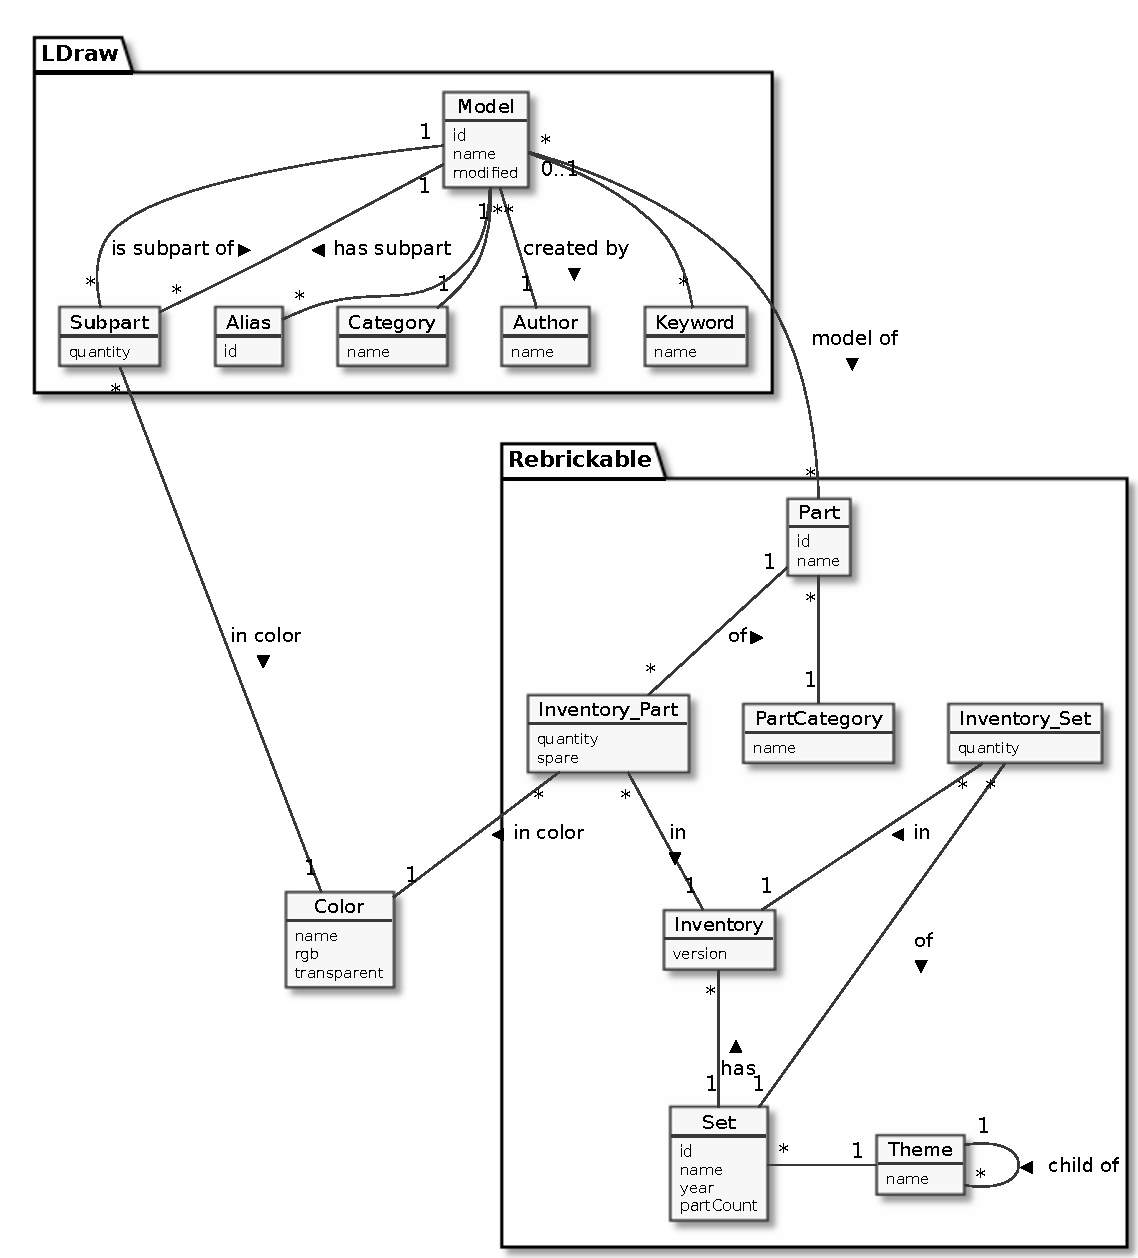
\includegraphics[width=\textwidth,height=\textheight,keepaspectratio]{pdfs/domain_ldraw_rebrickable}
    \caption{Doménový model: LDraw a Rebrickable\label{diagram-domenovy}}
  \end{figure}

\subsection{LDraw}
První balíček obsahuje entity týkající se součástek z~knihovny LDraw.

\subsubsection*{Model}
  Entita \textit{Model} (tabulka \emph{\ref{table:entity:model}}) reprezentuje jednu součástku z~knihovny LDraw. Atributy entity vychází z~dat obsažených v~jednotlivých souborech knihovny a ze specifikace hlavičky, která byla představena v~podsekci \emph{\nameref{ldraw-hlavicka}} sekce \emph{\ref{reserse-ldraw}}.
    
  U~každého \textit{Modelu} musí být evidován jeho autor z~důvodu možnosti dodržení licence \gls{CC-BY} \cite{CC-BY}, pod kterou jsou zveřejněny všechny součástky v~oficiální knihovně LDraw. 
  
  \begin{table}[th!]
  \centering
  \caption{Přehled atributů entity \textit{Model}}
  \label{table:entity:model}
  \begin{tabularx}{\textwidth}{@{}rX@{}}
  \toprule
  Atribut & Popis
  \\ 
  \midrule
  id: & Unikátní textový identifikátor modelu
  \\
  name: & Jméno modelu 
  \\
  modified: & Datum poslední úpravy modelu 
  \\
  partCount: & Počet součástek ve stavebnici
  \\
  path: & Cesta k~souboru 3D modelu na serveru
  \\
  \bottomrule
  \end{tabularx}
  \end{table}

\subsubsection*{Author}
Entita \textit{Author} reprezentuje autora, který svými modely přispívá do knihovny LDraw. Aby mohl být model zahrnut do oficiální knihovny, musí být autor registrován a projevit souhlas s~Dohodou přispěvatelů Ldraw.org \autocite{ldraw:agreement}.
  
\subsubsection*{Alias}
Entita \textit{Alias} reprezentuje alternativní identifikátor modelu, na který má vazbu. 

Uchování alternativních identifikátorů modelů slouží ke sjednocení tvarově identických součástek. Uchovávání každé součástky by z~hlediska 3D tisku nemělo žádný význam, protože jejich rozdíly (například potisk) zaniknou okamžikem převodu do formátu \textit{STL}.

\subsubsection*{Subpart}
Protože formát LDraw umožňuje i vytváření součástek typu \textit{Shortcut}, které jsou definovány v~podsekci \emph{\nameref{ldraw-typy-soucastek}} sekce \emph{\ref{reserse-ldraw}}, je nutné mít možnost uchovat informaci o~vztahu mezi jednotlivými modely. Toto je umožněno entitou \textit{Subpart}. 

Entita \textit{Subpart} kromě vazeb na \textit{Model} obsahuje atribut specifikující četnost výskytu podsoučástky a vazbu na entitu \textit{Color}, která specifikuje barvu. 

\subsubsection*{Category}
Každý model je zařazen do kategorie, která je určena v~hlavičce souboru.

\subsubsection*{Keyword}
K~možnosti vyhledávání v~knihovně LDraw mohou součástky a podsoučástky definovat klíčová slova.

\subsection{Rebrickable}
Druhý balíček sdružuje entity ze služby Rebrickable, která poskytuje inventáře součástek a stavebnic.

\subsubsection*{Set}
Entita \textit{Set} reprezentuje jednu stavebnici LEGO. Každá stavebnice má své unikátní id určené přímo společností LEGO. 

\subsubsection*{Part}
Entita \textit{Part} reprezentuje jednu unikátní součásku LEGO z~databáze Rebrickable.

\subsubsection*{Inventory}
Stavebnice může být během času vydána v~novější verzi, ve které je například vyměněna pouze jedna součástka. To vede k~potřebě zvláštní entity \textit{Inventory}, která reprezentuje tyto verze inventářů. 

\subsubsection*{Inventory\_Part} 
Součástky se ve stavebnicích mohou vyskytovat v~různých barevných provedeních. Dále je běžné, že stavebnice LEGO obsahují některé součástky navíc, které nejsou nezbytné k~jejich sestavení. Proto je v~nutná entita \textit{Inventory\_Part}, která umožňuje zaznamenání tohoto vztahu mezi součástkou a inventářem, včetně informace o~počtu, barvě a typu součástky.

\subsubsection*{Inventory\_Set}
Stavebnice se nemusejí skládat pouze ze součástek, ale mohou sdružovat i větší množství jiných stavebnic. Proto je nutná entita \textit{Inventory\_Set}, která reprezentuje tento vztah mezi stavebnicí a inventářem.

\subsubsection*{Theme}
Každá stavebnice náleží do série. Série je reprezentována entitou \textit{Theme}. Série může být zároveň podřazena jiné sérii. Zpravidla je zanoření maximálně tři úrovně hluboké.

\subsubsection*{Color} 
Entita \textit{Color} (tabulka \emph{\ref{table:entity:color}}) je společná pro oba balíčky. To je dáno faktem, že Rebrickable se svými daty vychází právě z~knihovny LDraw, jak bylo zmíněno v~sekci \emph{\ref{reserse-rebrickable}}.

\begin{table}[th!]
  \centering
  \caption{Přehled atributů entity \textit{Color}}
  \label{table:entity:color}
  \begin{tabularx}{\textwidth}{@{}rX@{}}
  \toprule
  Atribut & Popis
  \\ \midrule
  id: & Unikátní LDraw id barvy \autocite{ldraw:colors}
  \\
  name: & Jméno barvy
  \\
  rgb: & Hexadecimální \gls{RGB} kód barvy 
  \\
  transparent: & Indikátor o~transparentnosti barvy
  \\
  \bottomrule
  \end{tabularx}
\end{table}

\subsection{Brickset}
Třetí balíček popisuje strukturu dat dostupných přes Brickset \gls{API}.   

\begin{figure}[htbp]
    \centering
    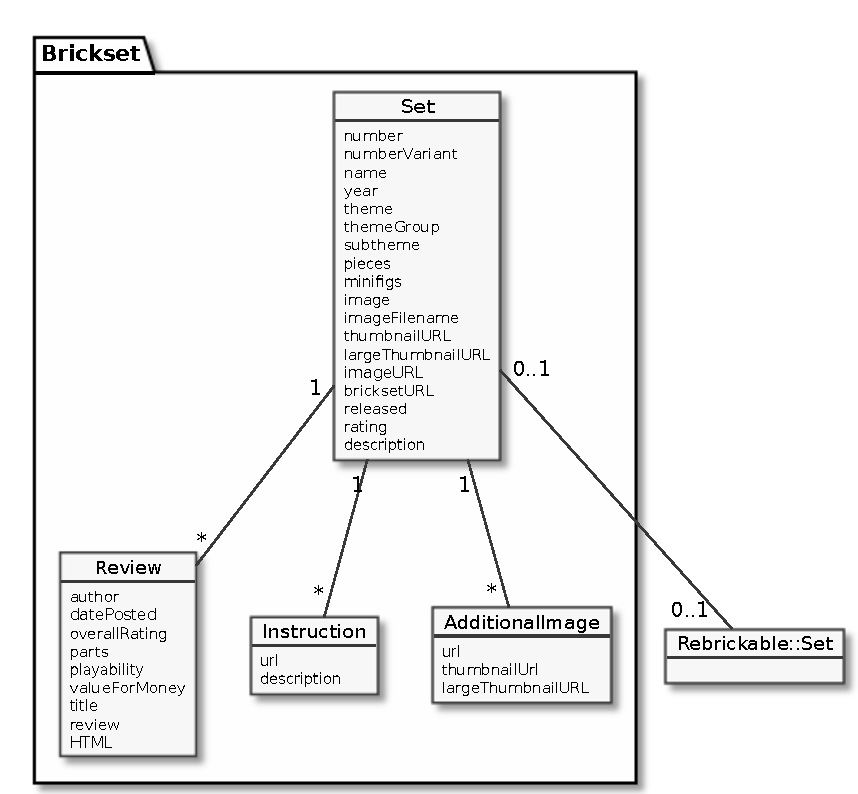
\includegraphics[width=\textwidth,height=\textheight,keepaspectratio]{pdfs/domain_brickset}
    \caption{Doménový model: Brickset \label{diagram-domenovy-brickset}}
\end{figure}

\subsubsection*{Set}
Entita \textit{Set} reprezentuje jednu stavebnici LEGO. Tato entita odpovídá právě jedné nebo žádné entitě \textit{Set} z~balíků Rebrickable.  

\subsubsection*{Review}
Brickset umožňuje uživatelům vytvářet recenze na stavebnice. Tyto recenze jsou reprezentovány entitou \textit{Review}. Recenze kromě textového popisu obsahuje i číselné hodnocení hlavních kritérií, znázorněných v~diagramu.

\subsubsection*{Instruction} 
Instrukce k~postavení stavebnice je reprezentována entitou \textit{Instruction}.

\subsubsection*{AdditionalImage} 
Entita \textit{AdditionalImage} reprezentuje jeden obrázek stavebnice. Obrázky jsou dostupné kromě původní velikosti i v~podobě miniatur.



\section{Uživatelské rozhraní}

\subsection{Domovská stránka}
Návrh domovské stránky (obrázek \emph{\ref{wireframe-hlavni}}) je velmi minimalistický. Stránka slouží pouze k~seznámení uživatele s~významem aplikace a k~navigaci na další stránky pomocí dvou velkých bloků umístěných pod úvodní fotografií. V pravém horním rohu se nachází vyhledávací pole, které umožňuje uživateli rychlou navigaci na součástky a stavebnice.

\begin{figure}[htbp]
    \centering
    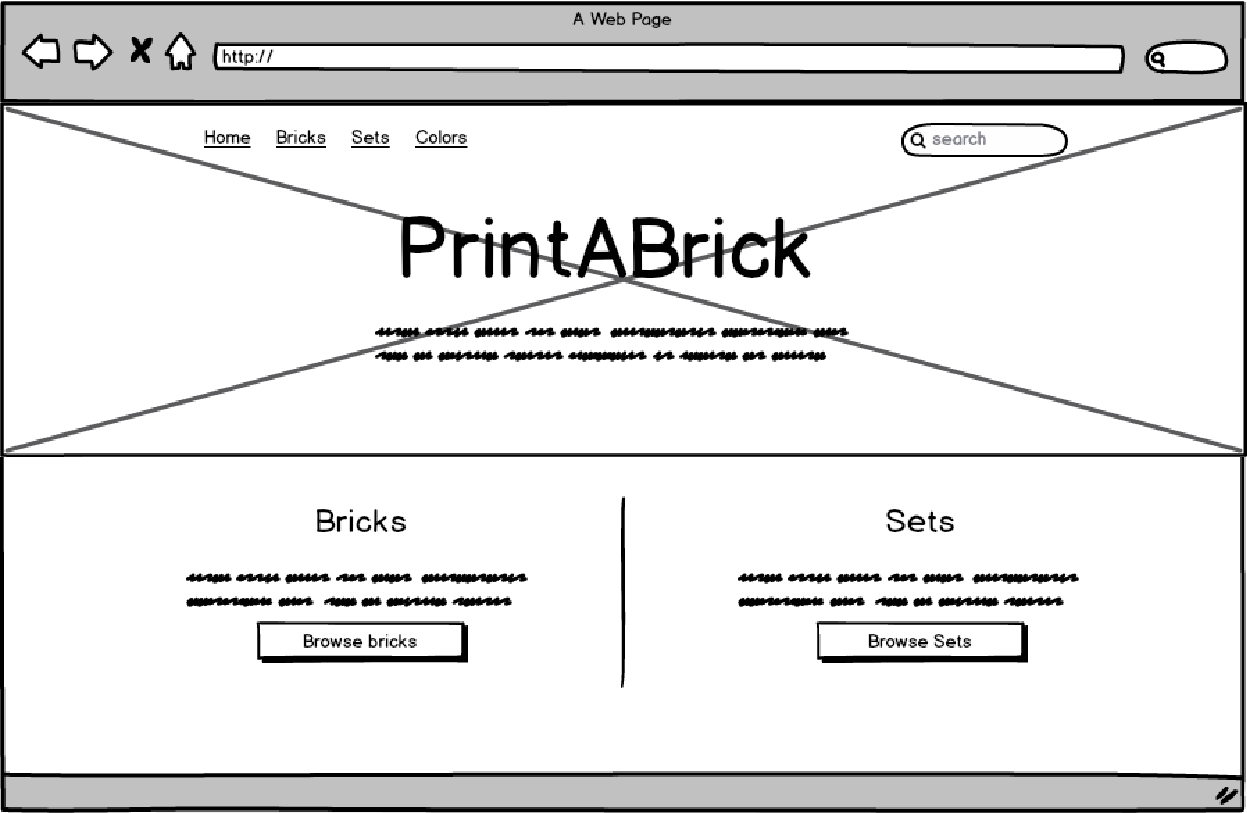
\includegraphics[width=\textwidth,height=\textheight,keepaspectratio]{pdfs/wireframe_home.pdf}
    \caption{Návrh hlavní stránky}\label{wireframe-hlavni}
\end{figure}


\subsection{Výpis stavebnic}
Na obrázku \emph{\ref{wireframe-stavebnice-seznam}} je možné vidět návrh stránky výpisu stavebnic. Tento výpis je stránkovaný a je možné ho řadit podle hlavních atributů stavebnic. Uživatel může specifikovat kritéria filtrování v~levém sloupečku. Sloupeček obsahuje textové pole pro zadání vyhledávaného výrazu, výběr kategorie a posuvníky určující počet součástek a rok vydání stavebnice.

Výpis stavebnic je zobrazen v~mřížce. Každý blok reprezentující stavebnici obsahuje obrázek a hlavní atributy, které mohou být uživateli nápomocné při výběru.

\begin{figure}[htbp]
    \centering
    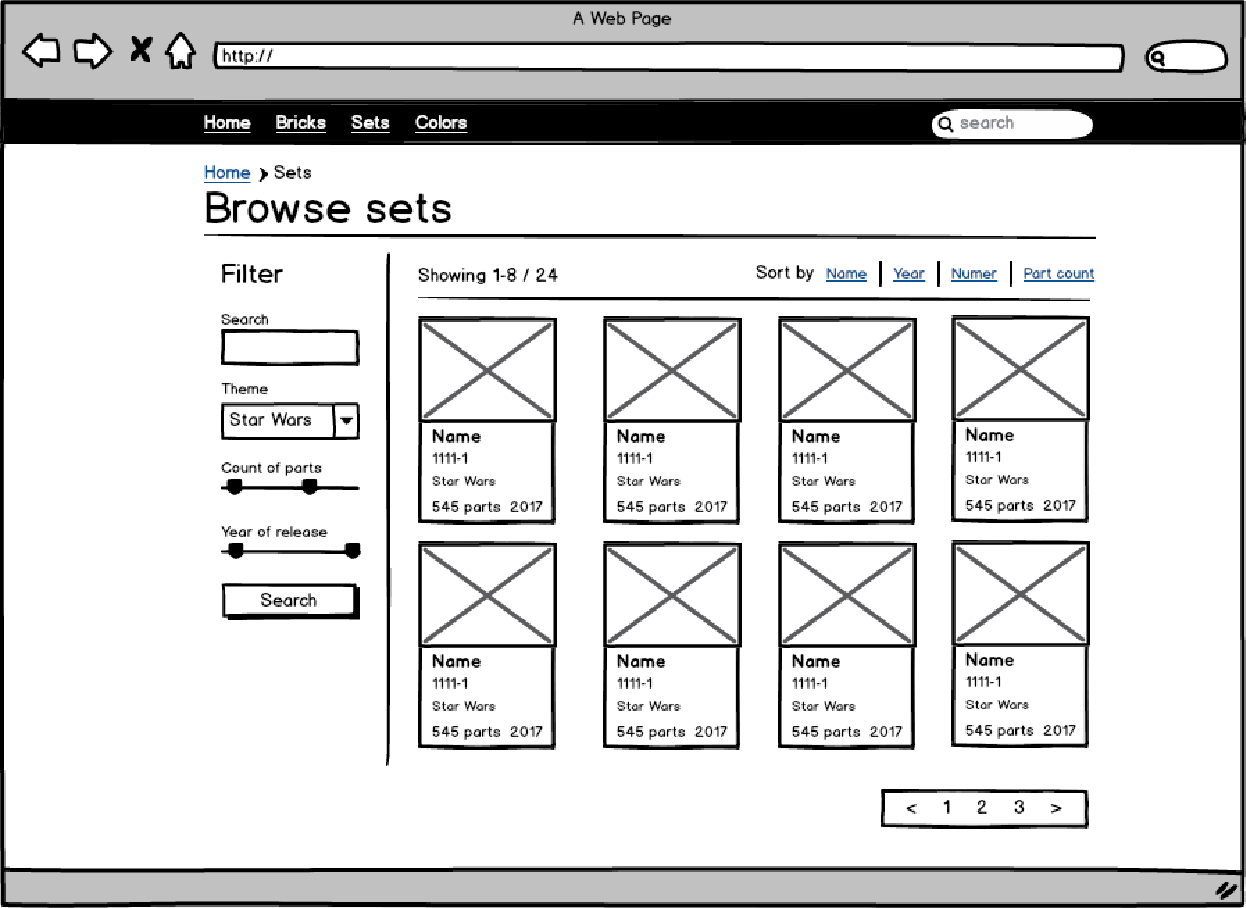
\includegraphics[width=\textwidth,height=\textheight,keepaspectratio]{pdfs/wireframe_sets.pdf}
    \caption{Návrh stránky výpisu stavebnic}\label{wireframe-stavebnice-seznam}
\end{figure}

\subsection{Výpis součástek}
Stránka výpisu součástek (obrázek \emph{\ref{wireframe-soucaska-seznam}}) je rozložením prvků navržena stejně jako stránka výpisu stavebnic. 

\begin{figure}[htbp]
    \centering
    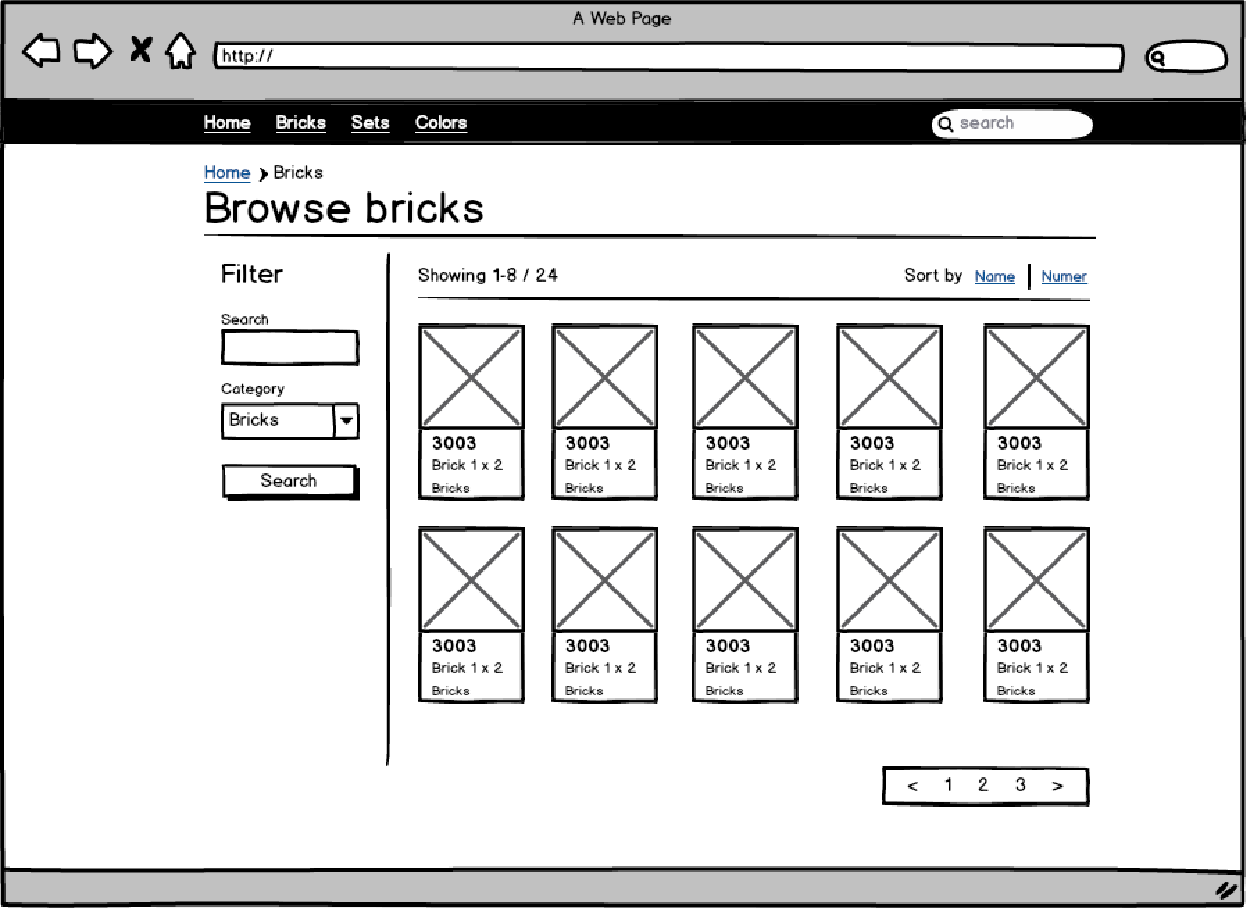
\includegraphics[width=\textwidth,height=\textheight,keepaspectratio]{pdfs/wireframe_bricks.pdf}
    \caption{Návrh stránky výpisu součástek}\label{wireframe-soucaska-seznam}
\end{figure}

\subsection{Detail stavebnice}
Stránka detailu stavebnice (obrázek \emph{\ref{wireframe-stavebnice-detail}}) představuje uživateli veškeré dostupné informace o~stavebnici. Stránka je grafiky rozdělena na dva bloky. 

Hlavní blok obsahuje obrázek stavebnice a atributy zobrazené v~tabulce. Dále obsahuje odkazy na služby ze kterých pochází zobrazená data.

Druhý blok je pro lepší přehlednost rozdělen do podstránek, které je možné přepínat pomocí horizontálního menu. Výchozí podstránkou je výpis součástek obsažených ve stavebnici. Tento výpis je možné zobrazit jak ve variantě ignorující barvy součástek, tak ve variantě roztříděné podle barev. Každá z~těchto variant obsahuje tlačítko pro stažení 3D modelů součástek.

Pokud pro stavebnici nejsou dostupné 3D modely všech součástek, je na stránce zobrazeno varování. 

\begin{figure}[htbp]
    \centering
    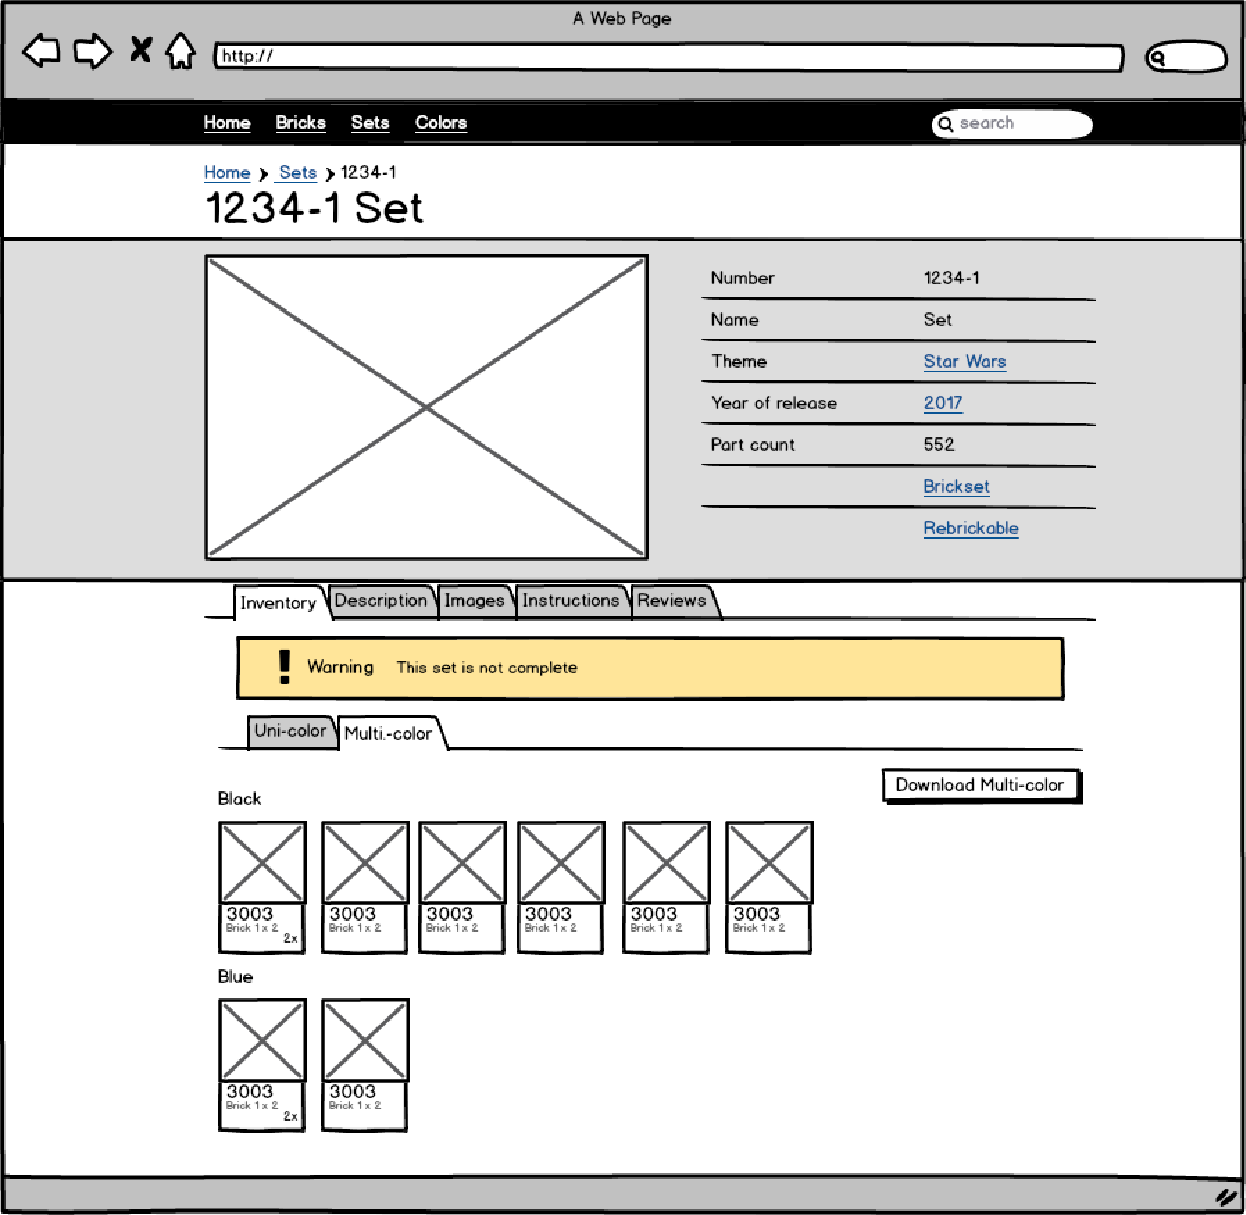
\includegraphics[width=\textwidth,height=\textheight,keepaspectratio]{pdfs/wireframe_set.pdf}
    \caption{Návrh stránky detailu stavebnice}\label{wireframe-stavebnice-detail}
\end{figure}

\subsection{Detail součástky}
Stránka detailu součástky (obrázek \emph{\ref{wireframe-soucastka-detail}}) je navržena podobně jako stránka detailu stavebnice. 

Hlavní blok obsahuje obrázek součástky a přehled atributů. Obrázek součástky má v~pravém horním rohu tlačítko, kterým se spouští interaktivní 3D náhled. Dále blok obsahuje tlačítko pro stažení 3D modelu. 

Druhý blok obsahuje dvě podstránky. První podstránka zobrazuje všechny příbuzné součástky. V~druhé je možné prohlížet veškeré stavebnice, ve kterých se součástka vyskytuje.

\begin{figure}[htbp]
    \centering
    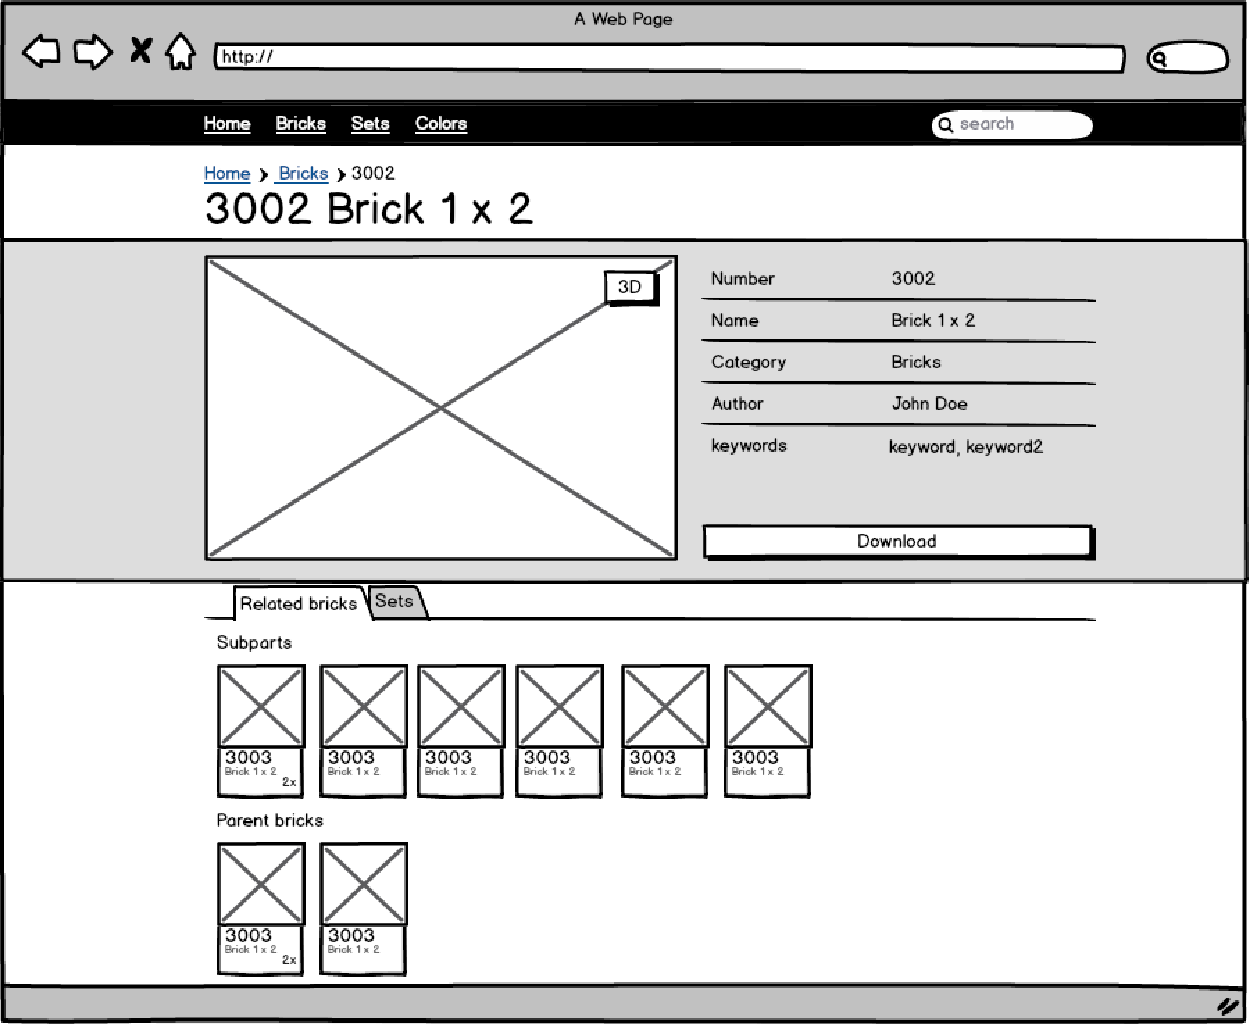
\includegraphics[width=\textwidth,height=\textheight,keepaspectratio]{pdfs/wireframe_brick.pdf}
    \caption{Návrh stránky detailu součástky}\label{wireframe-soucastka-detail}
\end{figure}

\subsection{Seznam barev}
Stránka seznamu barev (obrázek \emph{\ref{wireframe-barvy}}) slouží uživatelům k~seznámení se s~možnými barevnými variantami součástek. Barvy jsou zobrazeny ve dvou tabulkách. První tabulka sdružuje klasické barvy a druhá transparentní barvy. 

Tato stránka podle původního návrhu sloužila k možnosti dohledání přesné barvy součástky podle jména barvy. Později byla však tato informace zahrnuta přímo na místa, kde se vyskytuje zmínka o barvě. Tato stránka tedy postrádá svůj původní význam a mohla by být odstraněna.

\begin{figure}[htbp]
    \centering
    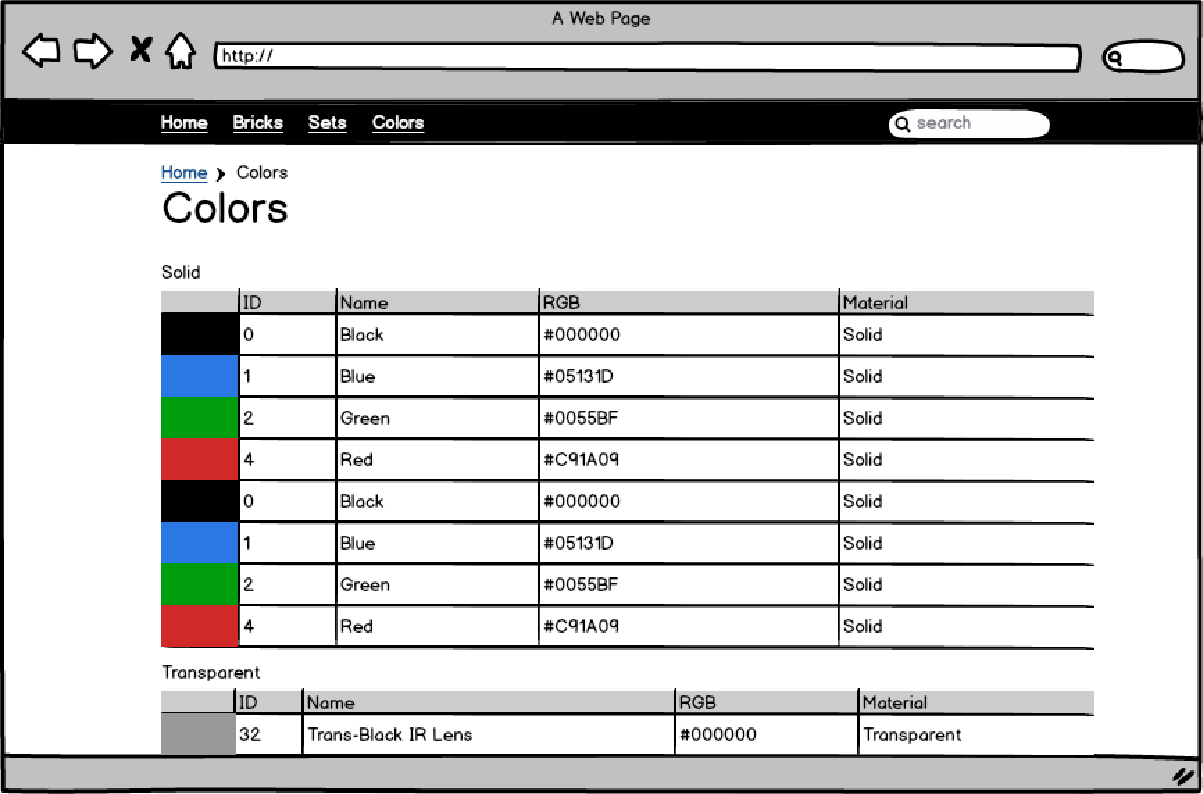
\includegraphics[width=\textwidth,height=\textheight,keepaspectratio]{pdfs/wireframe_colors.pdf}
    \caption{Návrh stránky seznamu barev}\label{wireframe-barvy}
\end{figure}

\chapter{Cíl práce}

\chapter{Rešerše}



\chapter{Implementace} 

\chapter{Právní aspekty} 

\chapter{Testování}
%TODO 
\begin{conclusion}
   

\label{conclusion}

\end{conclusion}

\printbibliography[title={Zdroje}]

\appendix

\chapter{Seznam použitých zkratek}
\printglossary[type=\acronymtype,style=acronyms]


\end{document}